
\subsection{Is Automated Monitoring Possible?}

It is entirely reasonable to ask whether automated monitoring,
including format inference and anomaly detection, is even
possible. Given that monitoring systems typically require explicit
configuration, automatic monitoring would present a significant
advance over the state of the art.

We have good reason to believe that our approach to automated
monitoring is possible for a wide variety of applications, especially
those that one would expect to encounter in a non-adversarial setting.
To understand the process, consider the following steps individually:

\begin{enumerate}
\item Isolating traffic flows and associating them with applications
\item Deriving formats and parsing data within flows
\item Detecting anomalous traffic
\item Querying archival data
\end{enumerate}

{\bf Isolating traffic flows} -- Assuming an appropriate network
vantage point that can see all relevant traffic, application flows can
be determined by noting that for most well-behaved application, port
selection is not random for one end of the connection. In a
client-server model, the client may choose a randomly-numbered
ephemeral port for communication, but the server's port is likely to
be something that's fixed across communications. This endpoint can be
determined either by observing the TCP handshaking process or by
observing port usage over time -- the fixed port is more likely to
appear across multiple flows than the random port. While some
applications, such as Skype or BitTorrent, may hop across ports to
reduce the chance of detection, our goal is to monitor the custom
network applications that are unlikely to have commercial monitoring
systems available. In contrast, VOIP or BitTorrent traffic can already
be tracked using commercially-available systems. Even other
applications that may have legitimate reasons for hopping ports may be
identifiable by deep packet inspection, which is part of our
system. Given the identification of flows, associating flows with
applications can be performed by having small stub programs running on
the servers to be monitoring. These stubs would use data from netstat
to identify which processes are associated with particular ports, and
could examine the process tree in the /proc pseudo-filesystem to trace
the processes to the applications that spawned them. Without these
stubs, the system would still be usable, but could only report traffic
types and port numbers, rather than application names.

{\bf Parsing Data} -- Once application flows have been isolated, the
contents of the flows can be examined to begin understanding the data
formats and parsing their contents. The main observation here is that
data sent on the wire is not likely to be random, but instead stem
from application needs. So, applications may send integers, or
strings, or floating-point numbers, and each of these formats has
characteristic bit patterns. Strings are likely to be centered around
the values representing characters rather than non-printing control
sequences. Integers are likely to be centered around popular numbers,
and IEEE floating-point numbers are likely to have specific patterns
in the mantissa and exponent.  Likewise, applications are not likely
to invent entirely new transport formats, so they may transfer raw
binary data for C programs, or marshalled serialized data for Java
programs, or data in particular representations (e.g., XDR) for
specific RPC protocols. Given enough examples of the data from the
applications, and given the space of known data formats, it is
possible to derive likely candidates for the format of the application
flows. These candidate formats can be exported to the operator for
refinement and naming with human-friendly labels, or they can be used
as-is. We intend to use the PADS system to describe the data flows,
which will present a high-level representation of the data which the
operator can modify as needed. By using PADS as the representation,
the rest of the PADS toolchain can be invoked, which will
automatically generate safe parsers for the data and generate
stand-alone tools that can be used to query the archives.

{\bf Detecting anomalies} -- Once the data streams can be parsed,
volumes of data can be collected for analysis, with the understanding
that applications are typically running without incident. By profiling
the data, statistical models can be derived for each field to
understand its typical behavior. Correlations between fields can also
be tested, and these expected values can be presented to the operator
in the same manner as the stream format gets presented. Over time,
tighter confidence intervals can be determined for the data, and when
the monitor encounters new data that is outside of the expected range,
it can raise alerts based on the magnitude of the deviation and the
sensitivity defined by the operator. The analysis can not only include
the data contained within the streams, but also the type of traffic
being handled. For example, if the monitor detects that a certain
record format that normally represents 1\% of the traffic is appearing
much more frequently, an alert can be raised on the frequency of the
record itself, rather than just on the data within the record. Where
possible, the operator or application developers are free to provide
information on the expected range of values and when alerts should be
raised, but even without augmentation, the montoring system can
determined its own baselines for each record. Note that this anomaly
detection is not guaranteed to be complete, but given the choice
between no monitoring or automatic inference, the inference may
provide a wealth of information that would otherwise be lost.

{\bf Querying Archives} -- Once a traffic anomaly has been reported by
the monitoring system, the operator can see what application was
involved, what data was transferred, and what the expected range of
values is for the underlying field. The monitoring system not only
archives the data in operation, but also archives the format
specification it has been using for that data. As a result, the
operator might see that field 3, which typically has a positive value,
is now negative. At this point, the application developer may wish to
augment the automatically-generated PADS specification with more
meaningful semantic information, such as replacing the label ``field
3'' with its true meaning. The on-line monitoring system can be used
to examine recent behavior of the traffic and can be used for simple
queries, while the PADS-generated tools can be run against the more
complete archive with arbitrarily complex queries. In doing so, the
developer can see the history of communication across the application
and the larger system, and can diagnose problems more easily by using
historical information rather than trying to reactively add new
instrumentation and hope that the problem recurs.

\subsection{Architecture and Infrastructure}


Two of the components of our system are PADS and CoMon, which not only
provide some of the necessary infrastructure for the internals of our
monitoring system, but which also provide benefits to the user-facing
portions of the system.  PADS provides a comprehensive system for
describing data in its native formats, and automatically generating
tools to access the data, both for live and archival data. CoMon works
with PADS to interactively present the data to operators, allowing
them to query it, view it graphically, and analyze trends on the data,
without having to provide manual configuration of the database.

Moving away from manual parsing simplifies the system and provides the
flexibility and security that hand-written parsers do not.  Given a
high-level specification, either provided by the operator or inferred
from the data, PADS will automatically generate a collection of
reliable, secure, and high-performance libraries as well as all of the
monitoring components, such as concurrently {\em ingesting/processing}
data from any number of distributed sources, {\em archiving}
(self-describing) data for later analysis, {\em querying} data to
troubleshoot problems, and {\em displaying} statistical data summaries
so users can monitor system health in real time.  As the system
changes and evolves, implementers can change the high-level
specifications and recompile to automatically obtain an improved
monitoring system.  In addition, since code is automatically
generated, as opposed to hand-written, it will not contain
vulnerabilities that make other systems susceptible to buffer
overflows and related attacks.  Finally, since PADS can describe the
format of any data source, users will be able to automatically
generate monitoring tools that interoperate with legacy software,
data, and devices.  Hence, our research can have an
immediate impact on the productivity of systems implementers by
helping produce the next generation of monitoring systems.  Overall,
our research will combine principled and innovative language design
with high-performance systems engineering, all aimed at solving
pervasive systems monitoring and measurement problems.



At the heart of such monitoring systems is a complex, multifaceted
data processing problem that involves, at a minimum, the following components.
\begin{enumerate}
\item collection, classification and aggregation of information 
distributed across the monitored system.
\item data archiving for later querying, measurement, security auditing and 
post-mortem forensic analysis
\item querying and information extraction from archived or current, online data
\item presentation and graphical display to administrators and users.
\end{enumerate}

A substantial part of the difficulty of building secure, reliable, efficient,
and evolving monitoring systems is the diversity, quality, and volume of data
these systems must often handle.  Often, new monitoring
systems face the problem of having to interact with legacy devices,
legacy software and legacy data, leaving implementers in a situation
where they cannot use robust off-the-shelf data management tools built for
standard formats like XML.  As a result, implementers simply
hack ``one-off'' monitoring tools of their own, which are invariably
less reliable, unoptimized, insecure, and difficult or impossible to evolve
when new requirements become known.

We call the nonstandard data formats that monitoring systems must
collect, aggregate, parse, print, archive, query, and present to 
users {\em ad hoc data formats}.   These formats, by definition,
have no standard data processing tools associated with them.
\figref{figure:data-sources} presents a selection of such formats
used in a variety of different monitoring systems.
They include ASCII, binary, and Cobol data formats, with
both fixed and variable-width records, ranging in size from
relatively small files through network applications which process over
a gigabyte per second.  Common errors in the data include undocumented data,
corrupted data, missing data, and multiple missing-value
representations.

\begin{figure*}
\begin{center}
\begin{tabular}{|l|l|l|l|l|}
\hline
Name \& Use   &  Representation              &Size           & Common Errors \\ \hline\hline
Web server logs (CLF): &  Fixed-column  & $\leq$12GB/week & Race conditions \\ 
Measuring web workloads         &  ASCII records &                 & on log entry \\
                                &                &                 & Unexpected values\\ \hline
CoMon data:              &  Geographically & 600 MB/day & Race conditions on\\ 
Monitor \& troubleshoot  &  distributed    & collected from           & log entry \\
PlanetLab infrastructure &  ASCII records  & \appr{}400-450 machines           & \\\hline
AT\&T provisioning data (\dibbler{}): & Variable-width  & 2.2GB/week & Unexpected values \\ 
Monitoring service activation & ASCII records  &            & Corrupted data feeds \\ \hline
Phone call detail:   &  Fixed-width   &\appr{}7GB/day &  Undocumented data\\ 
Fraud detection & binary records & & \\  \hline 
AT\&T billing data (\ningaui{}): & Various Cobol  & \appr{}4000 files/day, & Unexpected values\\ 
Monitoring billing process   & data formats            & 250-300GB/day    & Corrupted data feeds \\ \hline
IP backbone data (\darkstar{})  & ASCII  & $\ge$ 15 sources  & Multiple missing-value \\
Monitoring network performance  &        & \appr{}15 GB/day              & representations  \\ 
                                &        &                               & Undocumented data \\\hline
Netflow       & Data-dependent \# of     & $\ge$1Gigabit/second  & Missed packets\\ 
Monitoring network performance              &  fixed-width    &                       & \\ 
               & binary records & & \\ \hline
\end{tabular}
\caption{Selected ad hoc data sources for system monitoring. }
\label{figure:data-sources}
\end{center}
\end{figure*}

Processing this sort of 
ad hoc data is challenging for a variety of other reasons. 
First, when the data comes from legacy software, sources or devices, it 
typically just arrives ``as is'': the analysts
who receive it can only say ``thank you,'' not request a more
convenient format.  Second, documentation for the format may not exist
at all, or it may be out of date.  A common phenomenon is for a field
in a data source to fall into disuse.  After a while, a new piece of
information becomes interesting, but compatibility issues prevent data
suppliers from modifying the shape of their data, so instead they
hijack the unused field, often failing to update the documentation in
the process.

Third, such data frequently contain errors, for a variety of reasons:
malfunctioning equipment, race conditions on log entry~\cite{wpp},
non-standard values to indicate ``no data available,'' human error in
entering data, unexpected data values, \etc{} The appropriate response
to such errors depends on the application.  Some applications require
the data to be error free: if an error is detected, processing needs
to stop immediately and a human must be alerted.  Other applications
can repair the data, while still others can simply discard erroneous
or unexpected values.  For some applications, errors in the data can
be the most interesting part because they can signal where two systems
are failing to communicate.  Monitoring systems may need to respond to such
errors immediately and effectively.

Fourth, online monitoring systems
are highly susceptible to attack from malicious outsiders.
For example, intrusion detection systems
and performance evaluation systems that monitor network activity 
may be sent malicious packets or other data that cause buffer overflows
and allow attackers to take control of, evade, dismantle or corrupt these
systems.  A cautionary example of the dangers of online ad hoc data
processors is the Ethereal system~\cite{ethereal}. Ethereal is used by network administrators for monitoring, analyzing
and troubleshooting networks. Unfortunately, like most network software, users have found a number of
vulnerabilities in the software, and moreover many of these vulnerabilities are directly related to the mundane
components of the system that parse ad hoc data as opposed to the parts of the system that perform
higher-level tasks. For instance, in March 2004, Stefan Esser posted an advisory on 13 different buffer over-
flow attacks on Ethereal~\cite{etherealvulnerabilities}. Of the 13, 9 attacks occurred during parsing. These problems are not merely theoretical -- it was
a buffer overflow in a security monitoring system that was exploited by the
Witty Worm~\cite{witty}.

Fifth, ad hoc data sources can be high volume:
AT\&T's call-detail stream contains roughly 300~million calls per day
requiring approximately 7GBs of storage space. Although this data is
eventually archived in a database, analysts mine it profitably before
such archiving~\cite{kdd98,kdd99}. More challenging, the \ningaui{}
project at AT\&T accumulates billing data at a rate of 250-300GB/day,
with occasional spurts of 750GBs/day. Netflow data arrives from Cisco
routers at rates over a gigabyte per second~\cite{gigascope}! Such
volumes mean performance is critical and it certainly
must be possible to process the data without loading
it all into memory at once.

Finally, before anything can be done with an ad hoc data source,
someone has to produce a suitable parser for it.  Today, people tend
to use \C{} or \perl{} for this task.  Unfortunately, writing parsers
this way is tedious and error-prone, complicated by the lack of
documentation, convoluted encodings designed to save space, the need
to produce efficient code, and the need to handle errors robustly to
avoid corrupting downstream data.  Moreover, the parser writers'
hard-won understanding of the data ends up embedded in parsing code,
making long-term maintenance difficult for the original writers and
sharing the knowledge with others nearly impossible.

\paragraph*{Data-centric Monitor Generation}
We propose {\em data-centric monitor generation}, a new paradigm
for construction system monitors, in which programmers
specify the shape and properties of data manipulated by
the monitoring system and a compiler automatically
generates efficient, reliable, and secure
monitoring tools from that specification.
More specifically, the system will consist of the 
following components:

\begin{enumerate}

\item A high-level specification language to describe a monitor's
data sources.  The specification language will be able to
concisely and accurately describing any ad hoc data source,
including its format, semantic properties, location, and
temporal attributes in an easy-to-understand, easy-to-modify syntax.

\item A compiler that takes data specifications as inputs and
automatically generates a suite of 
efficient data processing libraries for parsing, printing, error detection
and correction, distributed data gathering, compression, and 
reformatting of ad hoc data.

\item A fully automatic tool generator that links the compiler-generated 
libraries to format-independent tool stubs to produce easy-to-use 
tools for high-level tasks including data display and querying.

\end{enumerate}

\begin{figure}[t]
\begin{center}
\centerline{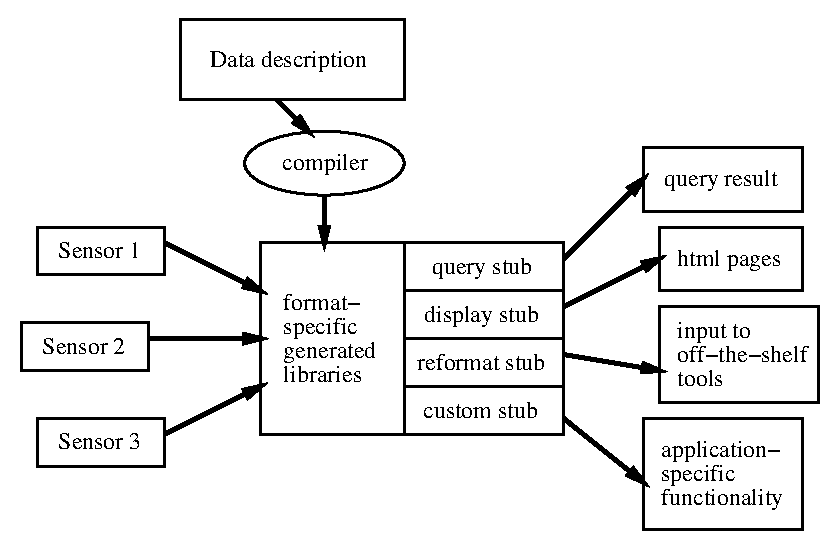
\psfig{file=arch_idraw_edit.ps,height=2.5in}}
\end{center}
\caption{\label{fig:arch} Architecture of Data-centric Monitor Generator.
}
\end{figure}

In the follow section, we will explain 
the architecture of a data-centric monitor generation system
and our prototype language design in more detail.  
Next, we will explain more of the specifics concerning
the generated tool suite for system monitoring.
In Section~\ref{ssec:features}, we will highlight some of the most
important language design challenges we face and
in Section~\ref{ssec:semantics}, we will propose a
formal system analysis to identify implementation errors
and improve system reliability.
In Section~\ref{ssec:impact}, we will explain how our research
on automatic generation of data processing tools
will make a broad impact on data processing that must be done
in disciplines well outside the bounds of
traditional computer science ranging from microbiology to physics to
economics.  We will also explain our education plan.

